
\documentclass[xcolor=x11names,compress]{beamer}


\usetheme[draft,num]{SmartSerif}

\usepackage{graphicx}
\DeclareGraphicsExtensions{.pdf,.png,.jpg}
\graphicspath{{./images/}}
\usepackage{color}

\usepackage{subcaption}



% ---------------------------------------------------------------------------------------
% Thanks to http://www.guidodiepen.nl/2009/07/creating-latex-beamer-handouts-with-notes/
 % \usepackage{handoutWithNotes}
 % \pgfpagesuselayout{4 on 1 with notes}[a4paper,border shrink=5mm]
 % \pgfpagesuselayout{2 on 1 with notes landscape}[a4paper,border shrink=5mm]
% ---------------------------------------------------------------------------------------

\setcounter{tocdepth}{2}

\title{Using Life-Logging to Re-Imagine Representativeness in Corpus Design}
\author{Stephen Wattam\\
Paul Rayson\\
Damon Berridge}
\institute[2013]{Lancaster University}
\date{\tiny \today}

\begin{document}

\maketitle

\frame{\frametitle{Contents}
    \tableofcontents
}




% -----------------------------------------------------------------------------------------
% \frame{\frametitle{Balance/Representativeness}
% 
%         % Representativeness is, simply:
%         Maximising the extent to which a sample resembles the population
% 
%         % For a given question 
%         % For a given population (needs defining)
% 
% 
%         \begin{itemize}
%             \item \textbf{Balance/Proportionality}---The ability of each sample to relate to its real-world counterpart
%                 % As seen in some given dimension
%                     
%             \item \textbf{Size}---The ability to adequately represent sub-populations fully for subsampling and specific inquiry
%                 % i.e. is there enough data on a given subtype of language?
%         \end{itemize}
% 
%         Language is so complex that, to satisfy these for a given research question, we require a very large sampe size
% 
% \note{}
% }
% 

% =============================================================================
\section{Sampling Design}

\subsection{Conventional}

\frame{\frametitle{Conventional Corpus Design}
    \begin{itemize} 
        \item Samples across a large population 
            \vspace{10pt}
            % i.e. books themselves, rather than the act of reading

        \item Stratified along genre, medium, etc.
            \vspace{10pt}
            % This differs from social science samples, who usually use variation across
            % the social population
            % 
            % There's a fair amount of disagreement on what variables are most important still
            %
            % It's not possible to sample consumption/production without having better information on these

        \item Based on available indexes such as bestseller lists
            \vspace{10pt}
            % i.e. bestseller lists, etc

        \item Tightly coupled to expert opinion on text importance
            % Which lists to use, etc, is chosen by committee
            % these have direct influence on content (selecting more books, for example)

    \end{itemize}

    \note{
        BNC: "Texts were chosen for inclusion according to three selection features: domain (subject field), time (within certain dates) and medium (book, periodical, etc.)."
    }
}

% 
% \frame{\frametitle{Difficulties}
%     \begin{itemize}
%         \item Many variables don't have indexes
%             \vspace{10pt}
%             % (i.e. production vs consumption)
%         \item Ethical or legal concerns limit some types of data
%             \vspace{10pt}
%             % i.e. speech vs writing proportions
%         \item Selection using `proxy variables', due to lack of auxiliary data
%             \vspace{10pt}
%             % and these have interactions with other variables of interest, i.e. p[in index list] correlates with some social/linguistic property
%         \item True empirical distribution of many variables is unknown
%             % leading to unrepresentative choices for stratum size
%             % such as time authored/read vs "was made in this year"
%     \end{itemize}
% 
%     \note{}
% }



% TODO: the slide below 
% \subsection{Literature}
% \frame{\frametitle{Literature}
%     \begin{itemize}
%         \item Biber
%         \item Varadi
%         \item Leech
%         \item
%     \end{itemize}
% \note{}
% }

% NOTE: another approach here would be to send out questionnaires in order to assess
%       the social validity of corpus results, i.e. to check the indexes.

\subsection{Personal}
\frame{\frametitle{Personal Corpus}
    \begin{itemize}

        \item All linguistic transactions 
            \vspace{10pt}
            % a language transaction, a la Leech
            %

        \item Expert opinion only needed to select demographics
            \vspace{10pt}
            % though sample size is still a hot topic and always will be
            % population is now "all users of x language",
            % the users can be determined through other surveys

        \item Opportunities for census of language genres
            % Constant recording can record everything, for once
            % Personal corpus stuff.

    \end{itemize}
    % \begin{itemize}
    %     \item 

    %     \item Selecting different variables of interest re-orients many practical issues
    %     % back to basics --- what is the aim of CL?
    %     \item I've chosen to sample language as a social, transitive, event
    %         % i.e. for a given group of people, what language do they use?
    %     \item Sample proportions of language use 'in the wild'
    %     \item With sufficient sample size, this is equivalent, however, pragmatic sampling issues differ greatly
    % \end{itemize}
\note{}
}


\frame{\frametitle{Advantages}
    \begin{itemize}
        \item Social demographics are well documented
            \vspace{10pt}
        \item No central index is required 
            \vspace{10pt}
            % The person is a central index
        \item Additional variables are exposed to study
            \vspace{10pt}
            % production/consumption, time/context etc.
            % more variables, i.e. not only author/title/genre (which may still be there),
            % but also social ones and transitive ones
        \item Discovery of language types/uses possible
            % ephemera, TV, labels, billboards etc

    \end{itemize}

\note{}
}


\frame{\frametitle{New Difficulties}
    \begin{itemize}
        \item Sampling text from many people is technically demanding, expensive
            \vspace{10pt}
            % We have to leave the office more
            % technology makes this easier nowadays
            % This is also an issue for things like the BHPS
        \item Size issues now affect `how many people'
            \vspace{10pt}
            % difficult even for simple data
            % dependent on the variability of people's everyday usage (a la biber)
        \item Multi-modal sources require transcription 
            % but this can be helped by using the sample as auxiliary data
            % Many things don't start of so well curated
    \end{itemize}
\note{}
}











% -----------------------------------------------------------------------------
\subsection*{Aims/RQs}
\frame{\frametitle{Aims}
Construct a personal corpus, to determine:

    \begin{itemize}
        \item What proportions of language types I use
        \item If any types of language are missing entirely from existing corpora (BNC)
            % Yes, Chomsky was correct ;-)
        \item Relative proportions of text and speech
        \item Practical methods for deployment using other subjects
        \item Time required to build a useful sample size
            %(based on variation seen, temporal cyclic stuff);
    \end{itemize}

% In addition to this, I have a number of studies planned using the data, but those can wait
\note{}
}

\frame{\frametitle{Process}
    \begin{itemize}
        \item Record \textit{all} language used (produced or received), in \textit{all} formats
            \vspace{10pt}
        \item Record for long enough to cover periodic effects
            \vspace{10pt}
        \item Compile daily lists of language types used
            \vspace{10pt}
        \item Transcribe and convert logs into a usable corpus
            % What constitutes long enough?
    \end{itemize}
\note{}
}










% =============================================================================
\section{Life-Logging}
% -----------------------------------------------------------------------------
\subsection*{History}
\frame{\frametitle{Life-Logging}
    \begin{itemize}
        \item Continual verbatim recording/broadcasting of life
        \item Originally for entertainment (JenniCam, Justin.tv)
        \item Heavily reliant on portable technology, connectivity

            \vspace{10pt}
            \begin{figure}
                \centering
                \begin{subfigure}[b]{0.5\textwidth}
                    \centering
                    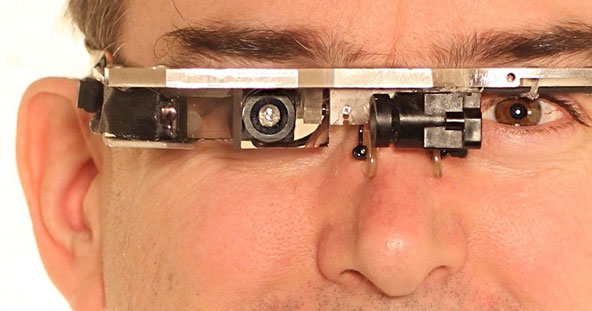
\includegraphics[width=\textwidth]{mann}
                \end{subfigure}%
                ~ %add desired spacing between images, e. g. ~, \quad, \qquad etc.
                %(or a blank line to force the subfigure onto a new line)
                \begin{subfigure}[b]{0.35\textwidth}
                    \centering
                    
\includegraphics[width=\textwidth]{jennicam}
                \end{subfigure}
            \end{figure}

    \end{itemize}
    \note{}
}


% -----------------------------------------------------------------------------
\subsection*{Application to Corpus Design}
\frame{\frametitle{Applications}
    \begin{itemize}
        \item Memory augmentation: Steve Mann, SenseCam, Machine Listening
            \vspace{10pt}
        \item Information retrieval: DARPA LifeLog
            \vspace{10pt}
        \item Language acquisition: Deb Roy
            \vspace{10pt}
        \item Corpus Building: LLC, BNC (sort of)
            \vspace{10pt}
        \item Posterity/Narcissism: Dymaxion Chronofile, JenniCam
    \end{itemize}
\note{
    BNC: "Recruits who agreed to take part in the project were asked to record all of their conversations over a two to seven day period."
    BNC: "Given that we were not attempting to represent the complete range of age and social groups within each region..."
}
}



% =============================================================================
% \section{Method}
% \frame{\frametitle{}
% 
%     \begin{center}
%     \sc \Large Preliminary Study 
%     \end{center}
% 
%     % TODO: slide needs some work
% \note{}
% }


% =============================================================================
\section{Data Collection}
% -----------------------------------------------------------------------------
\subsection*{Methods}
% What to record
% 'later lookup'/notes
% trade-off between seamlessness and comprehensiveness
\frame{\frametitle{Collection Strategy}
    \begin{itemize}
        \item Focus on unobtrusive, recall-based logging
            \vspace{10pt}

        \item Daily journal of language use:
            \begin{itemize}
                \item Listings of language used
                \item Subjective descriptions of which sections were read
                \item Details of complex interactions (shopping, music)
                \item Annotation of daily continuous logs
            \end{itemize}

    \end{itemize}
\note{}
}

% Methods (one slide each?)
%  - technical
%   - squid
%   - recording (a/v)
%   - blog
%   - notebook
\frame{\frametitle{Data Sources}

%may be retrieved easily and need not be recorded verbatim
    \begin{itemize}
        \item Persistent (books, music, audio/video, notes)
            \vspace{10pt}
        \item Ephemeral (speech, adverts, todo lists)
            \vspace{10pt}
        \item Digital origin (documents, presentations, websites, emails, chat logs)
            \vspace{10pt}
    \end{itemize}

\note{}
}







% -----------------------------------------------------------------------------
\subsection*{Data Sources}

\frame{\frametitle{Journal}
The journal is formed from a physical notebook:

\begin{center}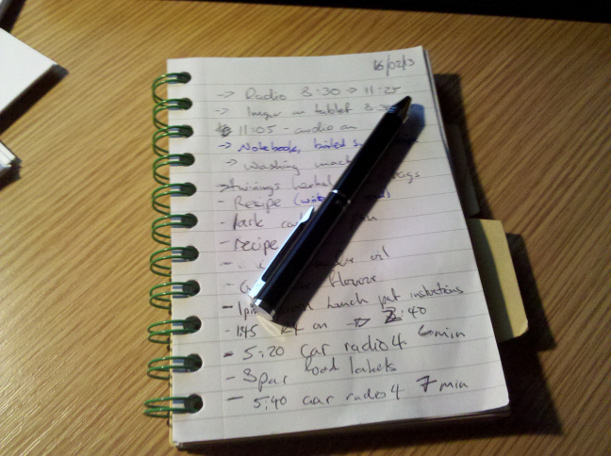
\includegraphics[width=3cm,height=2cm]{notebook}\end{center}

And an online log, which contains more detail:

    \begin{itemize}
        \item Details of complex activities I'm likely to forget
            %(items bought at shops, etc)
        \item Subjective estimates of proportions read from various sources
            %(web pages, books, etc)
    \end{itemize}
\note{}
}


\frame{\frametitle{Audio Recording}

\begin{center}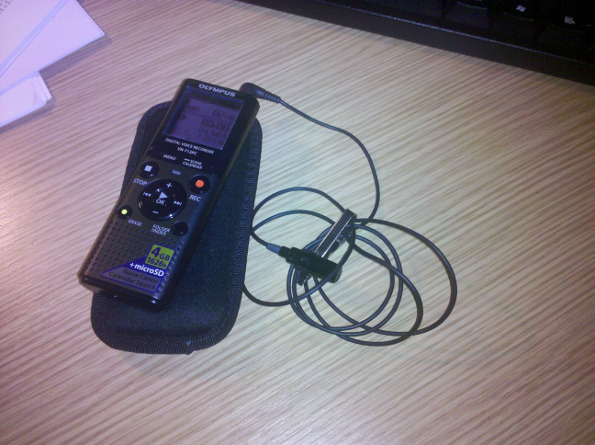
\includegraphics[width=4cm]{dictaphone}\end{center}
    
    \begin{itemize}
        \item Allows capture of small-scale speech events
        \item Difficult to process post-hoc without index markers, but realtime annotation is harder
        \item The law prevents external access without consent
    \end{itemize}

    \pause

 \begin{center}\alert{Ethical issues abound!}\end{center} 
\note{}
}

% 
% \frame{\frametitle{Video Recording}
% 
% \begin{center}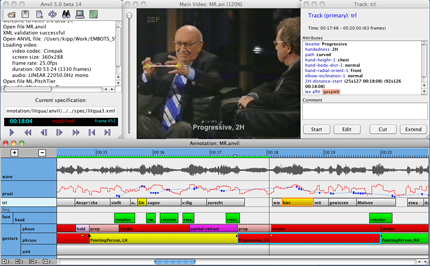
\includegraphics[width=4cm]{anvil5}\end{center}
% 
%     \begin{itemize}
%         \item Detailed multi-media recording for awkward situations
%         \item Useful when driving for road signs, music, GPS instructions, etc.
%         \item Difficult to annotate without 100\% time overhead
%     \end{itemize}
% \note{}
% }
% 
 \frame{\frametitle{Technical---Web}
\begin{center}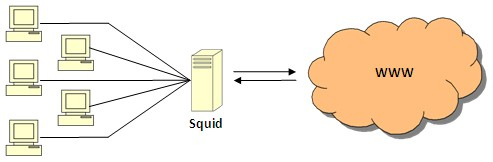
\includegraphics[width=7cm,height=2cm]{squid}\end{center}
    \begin{itemize}
        \item SQUID Proxy logs all traffic from my devices
        \item Heavy post-processing necessary:
            \begin{itemize}
                \item Removal of AJAX, automated, unread data
                \item Filtering of tags, boilerplate
                \item Removal of unread sections of text
            \end{itemize}
        \item A bot monitors web chat when I start speaking, and only logs when I am active
    \end{itemize}
\note{}
}

\frame{\frametitle{Technical---Other Digital Resources}
\begin{center}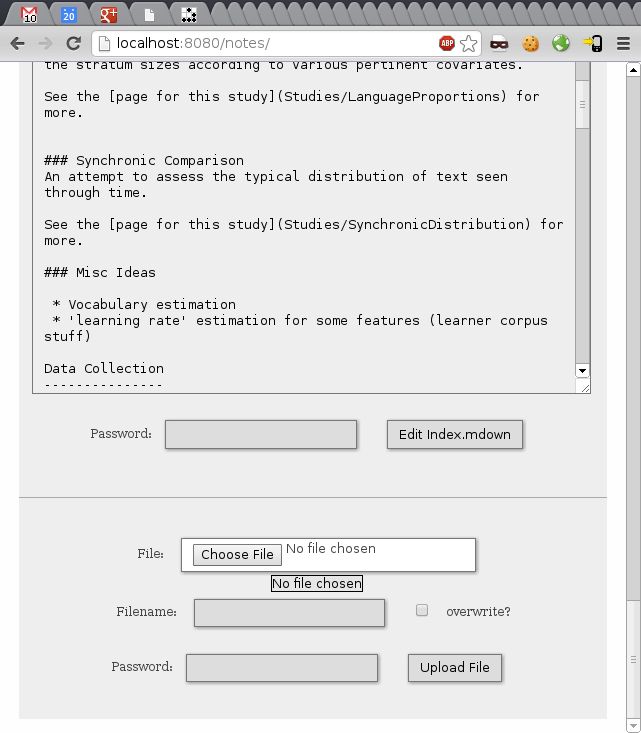
\includegraphics[width=3cm]{wik}\end{center}

    \begin{itemize}
        \item The journal and file store are accessible via the web
        \item Any files can simply be uploaded, or
        \item A flash drive can be used for large files
    \end{itemize}
\note{}
}


\frame{\frametitle{Technical---Input}
\begin{center}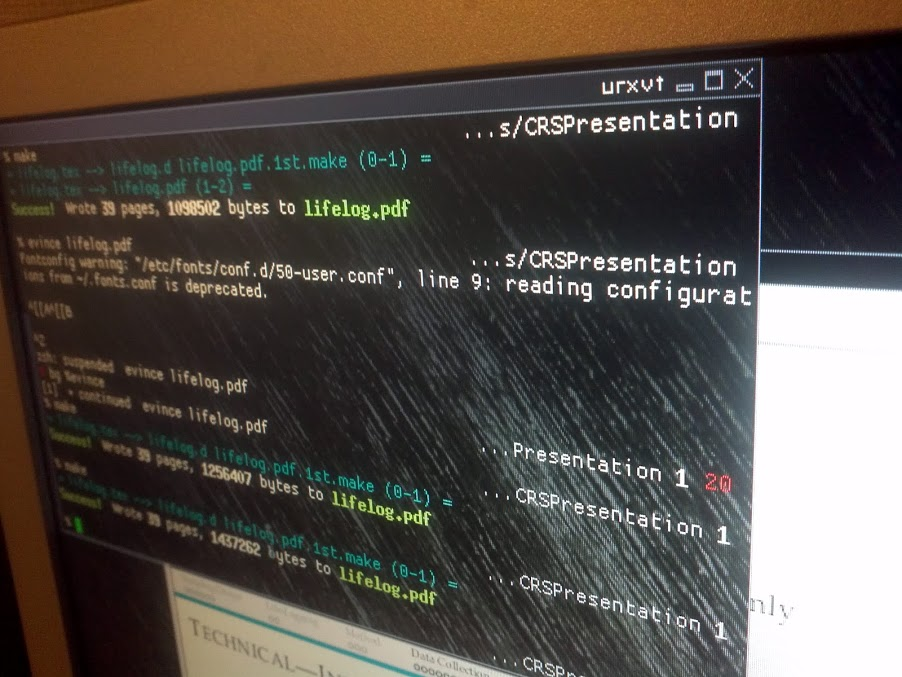
\includegraphics[width=4cm]{terminal}\end{center}
    \begin{itemize}
        \item Terminal-logging software can record all CLI use
        \item Keyloggers can capture all input, but often lack context information
        \item Email, web chat, other documents are all logged and timestamped
    \end{itemize}
\note{}
}

\frame{\frametitle{Digitisation}

\begin{columns}[t]
    \column{.6\textwidth}

        \begin{itemize}
            \item Cameraphone for billboards and packages
            \vspace{5pt}
            \item Thanks to tumblr, no-one cares that I'm taking a photo of some cereal packets in public
            \vspace{5pt}
            \item Longer documents can usually be scanned
        \end{itemize}

    \column{.4\textwidth}
        \begin{center}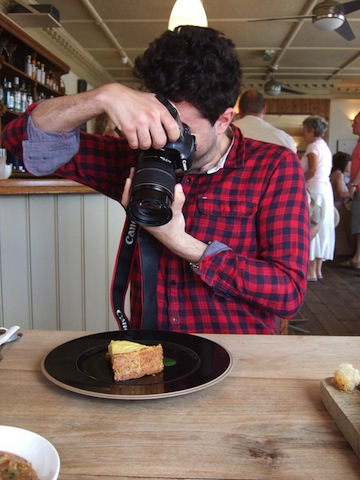
\includegraphics[width=4cm]{food-blogger}\end{center}
\end{columns}

\note{}
}













% -----------------------------------------------------------------------------
\section{Processing} 
% How to convert and transcribe data from disparate sources
% information processing, organisation, markup
\frame{\frametitle{Operationalisation}
    \begin{itemize}
        \item Only `easily lost' data is transcribed during the study (daily)
            \vspace{5pt}
        \item Variable selection deliberately small to minimise intrusiveness
            \vspace{5pt}

        \item Audio, Video are most problematic
            \vspace{5pt}

        \item Data stored centrally for easy lookup

        % \item Digital documents require significant post-processing to remove unread content
        %     % markup, or simply bits I don't read of web pages
        %     % most terminal output is unread
        %     % I'm not *always* reading web chat
        % \item Audio needs to be annotated for genre, particpant count, etc. or transcribed
        % \item Pictures require transcription
        % \item Notebook metadata needs tabulating (and, in many cases, completing)
        % \item Web logs need downloading, post-processing
    \end{itemize}
\note{}
}

\frame{\frametitle{Processing}
    \begin{itemize}
        \item Problems of simultaniety, attention
            \vspace{5pt}
        \item Processing tools contain a human interest model 
            \vspace{5pt}

        \item Manual coding of genre, manual correction of others
            \vspace{5pt}

        \item Custom scripts for pretty much everything
            % 2k lines of ruby

        % \item Digital documents require significant post-processing to remove unread content
        %     % markup, or simply bits I don't read of web pages
        %     % most terminal output is unread
        %     % I'm not *always* reading web chat
        % \item Audio needs to be annotated for genre, particpant count, etc. or transcribed
        % \item Pictures require transcription
        % \item Notebook metadata needs tabulating (and, in many cases, completing)
        % \item Web logs need downloading, post-processing
    \end{itemize}
\note{}
}









% 
% % =============================================================================
% \section{Use} 
% % -----------------------------------------------------------------------------
% \subsection*{Use}
% % Use as auxiliary data
% % Resampling
% % The idea of gathering more people's info
% % Digital-only corpora for web scraping and rabalancing
% % subject-specific corpora
% \frame{\frametitle{Direct Use}
%     \begin{itemize}
%         \item NLP models for `custom' interaction with devices and services
%             \vspace{5pt}
%             % google's personal search, sat nav
%         \item Balancing of corpora to specific demographics or people
%             \vspace{5pt}
%         \item Contextualisation of utterances with peer groups, etc
%             \vspace{5pt}
%         \item Comparison to existing language resources
%             \vspace{5pt}
%         \item Application to theories of lexical priming, language acquisition
%     \end{itemize}
% \note{}
% }
% 
% \frame{\frametitle{Methods for auxiliary data}
%     \begin{itemize}
%         \item Conventional corpora may be resampled to build a larger corpus
%             \vspace{10pt}
%         \item Inspecting similar demographics from existing corpora indicates the differences in bias between both methods
%         % T ODO
%     \end{itemize}
% \note{}
% }
% 
% 




% =============================================================================
\section{Data}
\subsection{Summary}


\frame{\frametitle{Data---Overview}
\begin{figure}
  \makebox[\textwidth][c]{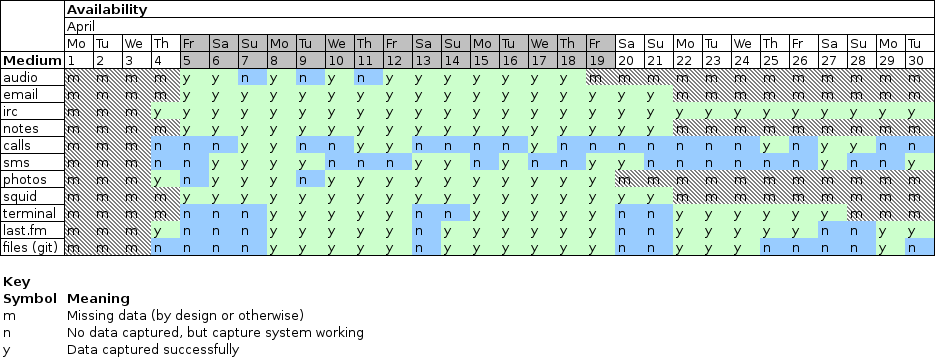
\includegraphics[width=1.15\textwidth]{dates}}%
  \label{fig:dates}
\end{figure}

    \begin{itemize}
        \item 15 days with full availabilty
            \vspace{5pt}
        \item $8,619$ linguistic events, $1.4$m words (est.), 3.4GB
        % T ODO
    \end{itemize}
\note{}
}




\frame{\frametitle{Data---Word Counts}
\begin{figure}
  \makebox[\textwidth][c]{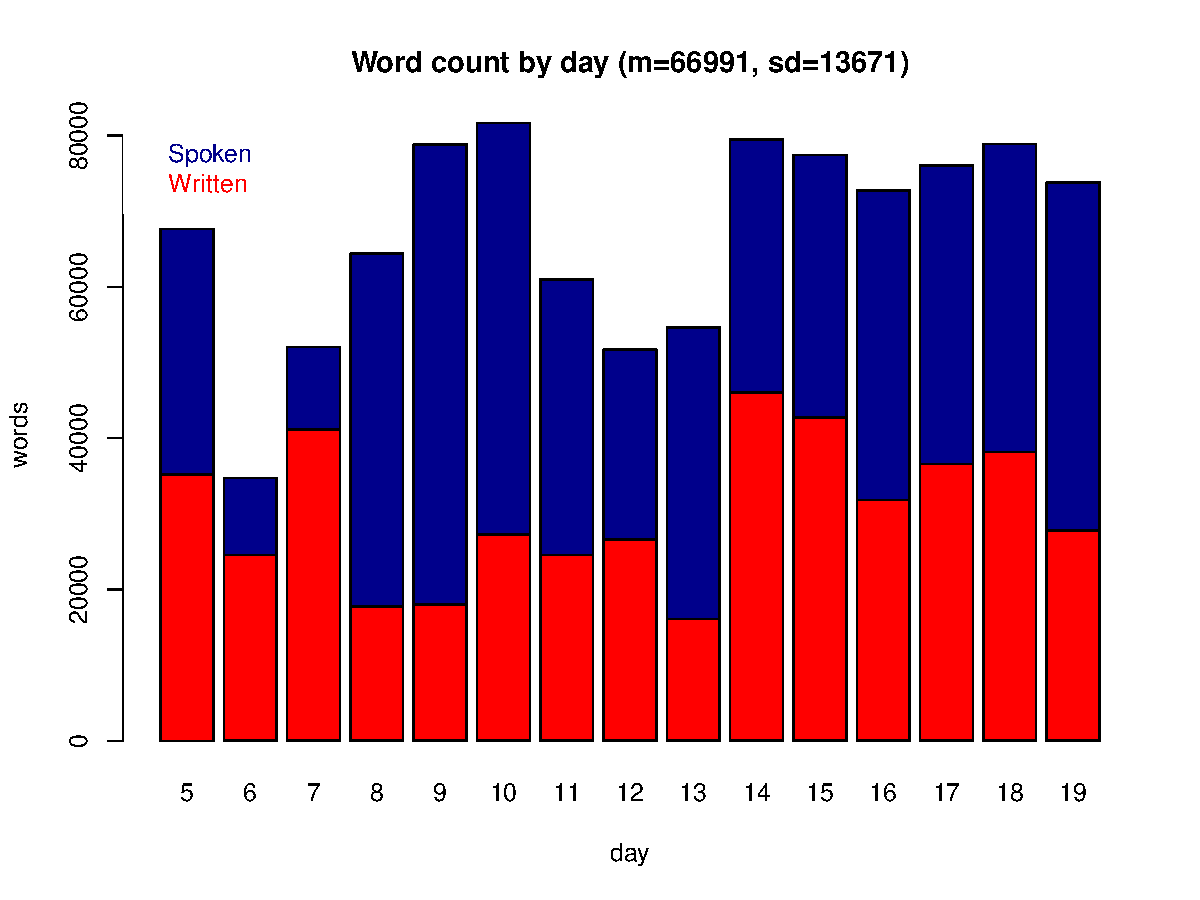
\includegraphics[width=\textwidth]{cbyday}}%
  \label{fig:dates}
\end{figure}
\note{}
}



\frame{\frametitle{Data---Production/Reception}
\begin{figure}
  \makebox[\textwidth][c]{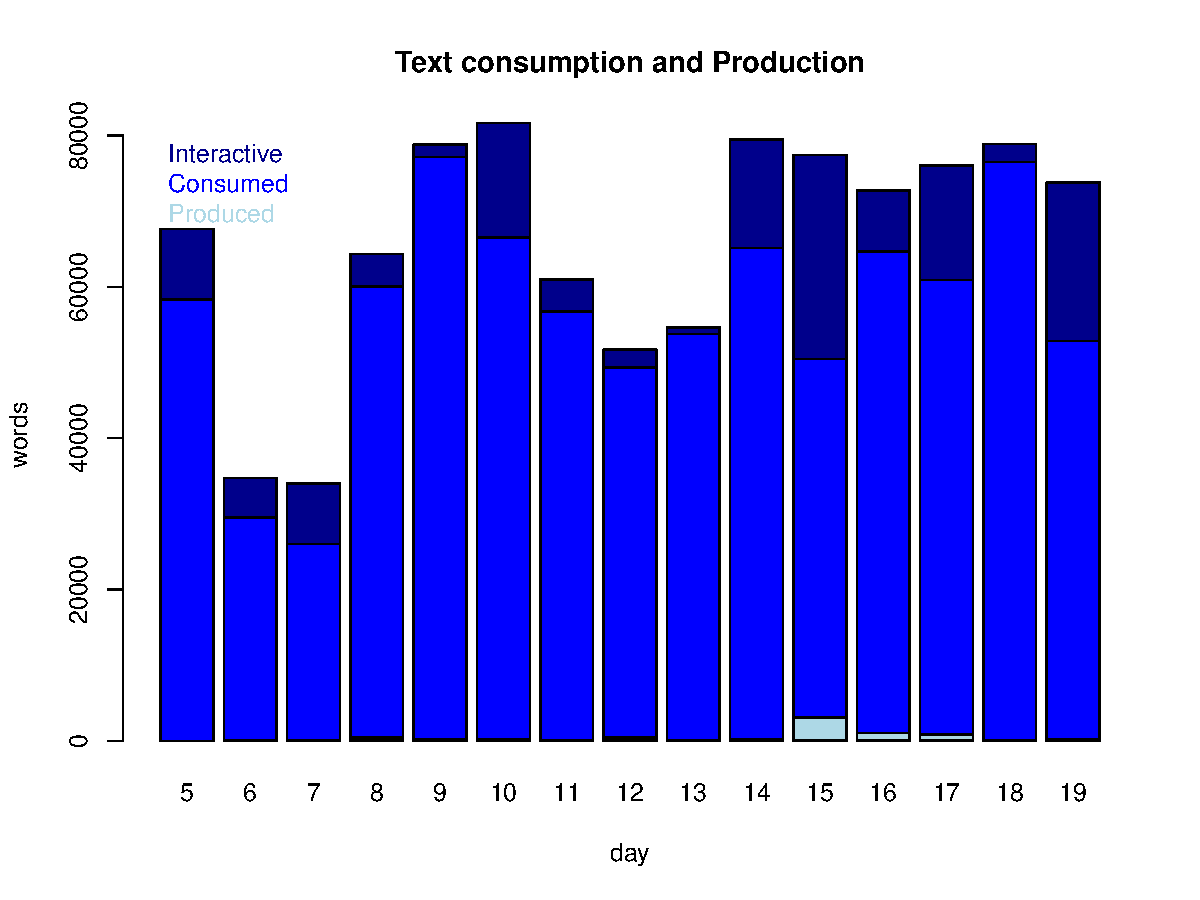
\includegraphics[width=0.9\textwidth]{prodbyday}}%
  \label{fig:dates}
\end{figure}

\tiny
\begin{center}
    85\% consumed (95\% of events), 15\% interactive (4\% of events), 0.6\% produced (0.5\% of events) 
\end{center}
\note{}
}




\frame{\frametitle{Data---Media}
\begin{columns}
    \column{.82\textwidth}
        \begin{itemize}
            \item Most written data online
                \vspace{10pt}
            \item Music is a surprisingly large component
                \vspace{10pt}
            % \item I use IRC more than I speak to people in real life
            %     \vspace{10pt}
            \item 45\% spoken, 55\% written
                \vspace{10pt}
            \item Reassuringly Zipfian distribution by event, day, genre, medium 
            % \item 
            %     \vspace{10pt}
                % \item ~3 hours of radio 4
        \end{itemize}


\begin{figure}
  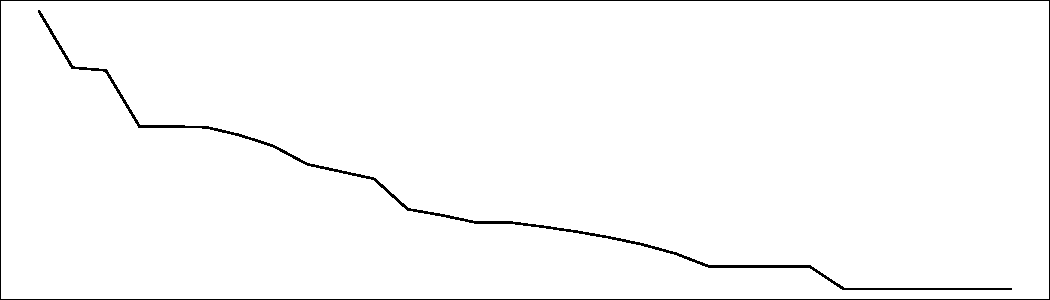
\includegraphics[width=0.8\textwidth]{distraw}%
\end{figure}


        \column{.18\textwidth}

        \tiny
        \vspace{-20pt}

        \begin{table}[ht]
            \centering
            \begin{tabular}{rr}
                web & 5828 \\ 
                music & 1000 \\ 
                display & 914 \\ 
                file & 159 \\ 
                irc & 159 \\ 
                email & 155 \\ 
                speech & 121 \\ 
                TV &  86 \\ 
                product &  49 \\ 
                sign &  39 \\ 
                radio &  31 \\ 
                flyer &  12 \\ 
                book &  10 \\ 
                application &   8 \\ 
                sms &   8 \\ 
                notes &   7 \\ 
                phone &   6 \\ 
                box &   5 \\ 
                poster &   4 \\ 
                paper slip &   3 \\ 
                game &   2 \\ 
                map &   2 \\ 
                vehicle &   2 \\ 
                video &   2 \\ 
                card &   1 \\ 
                cheque &   1 \\ 
                clothing &   1 \\ 
                film &   1 \\ 
                noticeboard &   1 \\ 
                taxdisc &   1
            \end{tabular}
        \end{table}


    \end{columns}

    \note{}
}



% 
% > sum(fn$computed_words_produced)
% [1] 6672.9
% > sum(fn$computed_words_consumed)
% [1] 859373.5
% > sum(fn$computed_words_interactive)
% [1] 138821.1
% > sum(fn$computed_words)
% [1] 1004868
% 
% > summary(fn$produced.consumed)
%    c    p   pc 
% 8156   44  418 
% > n = 8156 + 44 + 418
% > n
% [1] 8618



\frame{\frametitle{Data---Genre}



\begin{columns}
    \column{.7\textwidth}
        \begin{itemize}
            \item imgur.com has a lot to answer for(!) 
                \vspace{10pt}
            \item TV, email, and various websites feature
                \vspace{10pt}
            \item More obvious features of various activities
                \vspace{10pt}
            % \item 45\% spoken, 55\% written
            %     \vspace{10pt}
            \item Again, Zipfian around my interests
            % \item 
            %     \vspace{10pt}
                % \item ~3 hours of radio 4
        \end{itemize}


\begin{figure}
  
\includegraphics[width=0.8\textwidth]{gdistraw}%
\end{figure}


        \column{.3\textwidth}

        \tiny
        \vspace{-30pt}


        \begin{table}[ht]
            \centering
            \begin{tabular}{rr}
                web/entertainment/social & 2598 \\ 
                web/music & 708 \\ 
                display/output & 627 \\ 
                music/punk & 587 \\ 
                web/reference & 421 \\ 
                web/shopping & 388 \\ 
                display/interactive & 285 \\ 
                web/academic & 280 \\ 
                web/tech & 218 \\ 
                web/outdoors & 180 \\ 
                web/video streaming & 167 \\ 
                irc/informal/discussion & 159 \\ 
                music/guitar & 147 \\ 
                web/academic/reference & 142 \\ 
                web/tech/reference & 116 \\ 
                web/news & 105 \\ 
                file/ruby code &  82 \\ 
                music/metal &  73 \\ 
                music/pop &  68 \\ 
                music/rock &  67 \\ 
                web/hosting &  54 \\ 
                file/documentation &  49 \\ 
                web/comedy &  49 \\ 
                web/social &  49 \\ 
                web/product support &  48 \\ 
                product/packaging &  43 \\ 
                web/tech/academic &  40 \\ 
                TV/comedy &  39 \\ 
                web/outdoors/reference &  36 \\ 
                email/academic &  34 \\ 
                email/advertising &  28 \\ 
                web/entertainment &  28 \\ 
                \ldots & \ldots \\
                % email/personal &  26 \\ 
                % file/config &  24 \\ 
                % email/business &  22 \\ 
                % speech/discussion &  22 \\ 
                % speech/informal &  21 \\ 
                % web/comedy/social &  21 \\ 
                % email/orders &  20 \\ 
                % speech/service &  19 \\ 
                % web/search &  19 \\ 
                % email/spam &  17 \\ 
                % music/blues &  17 \\ 
                % speech/greeting &  16 \\ 
                % web/fitness &  16 \\ 
                % web/tech/news &  15 \\ 
                % TV/Entertainment &  14 \\ 
                % speech/info &  14 \\ 
                % web/tech/shopping &  14 \\ 
                % web/reference/academic &  13 \\ 
                % TV/news &  12 \\ 
                % radio/music &  12 \\ 
                % radio/news &  12 \\ 
                % sign/info &  11 \\ 
                % web/art &  11 \\ 
                % web/music/shopping &  11 \\ 
                % music/folk/metal &   9 \\ 
                % music/progressive &   9 \\ 
                % TV/entertainment &   8 \\ 
                % email/technical &   8 \\ 
                % sign/info/instruction &   8 \\ 
                % speech/ephemera &   8 \\ 
                % web/banking &   8 \\ 
                % music/country/rock &   7 \\ 
                % music/fusion &   7 \\ 
                % sign/product info &   7 \\ 
                % book/info &   6 \\ 
                % sign/advertising &   6 \\ 
                % TV/documentary &   5 \\ 
                % flyer/advertising &   5 \\ 
                % notes/note &   5 \\ 
                % product/info &   5 \\ 
                % speech/parting &   5 \\ 
                % web/advertising &   5 \\ 
                % web/conspiracy &   5 \\ 
                % box/address &   4 \\ 
                % flyer/info/advertising &   4 \\ 
                % radio/news/entertainment &   4 \\ 
                % sms/informal &   4 \\ 
                % web/blogs &   4 \\ 
                % web/games &   4 \\ 
                % web/news/social &   4 \\ 
                % web/reference/social &   4 \\ 
                % web/reference/travel &   4 \\ 
                % web/reference/woodwork &   4 \\ 
                % web/shopping/investment &   4 \\ 
                % web/tech/utility &   4 \\ 
                % web/utility &   4 \\ 
                % TV/advertising &   3 \\ 
                % application/info &   3 \\ 
                % file/js code &   3 \\ 
                % flyer/menu &   3 \\ 
                % music/country &   3 \\ 
                % phone/ &   3 \\ 
                % sign/advertising/info &   3 \\ 
                % sms/info &   3 \\ 
                % speech/organisation &   3 \\ 
                % speech/request &   3 \\ 
                % web/health &   3 \\ 
                % web/news/tech &   3 \\ 
                % application/info/status &   2 \\ 
                % book/packaging/book title &   2 \\ 
                % map/info &   2 \\ 
                % music/indie &   2 \\ 
                % paper slip/invoice &   2 \\ 
                % phone/informal &   2 \\ 
                % poster/advertising &   2 \\ 
                % radio/News &   2 \\ 
                % speech/Discussion &   2 \\ 
                % speech/informal/discussion &   2 \\ 
                % web/comedy/entertainment &   2 \\ 
                % web/entertainment/images &   2 \\ 
                % web/entertainment/news &   2 \\ 
                % web/entertainment/puzzles &   2 \\ 
                % web/game &   2 \\ 
                % web/tech/social &   2 \\ 
                % TV/advertising/info &   1 \\ 
                % TV/documentary/entertainment &   1 \\ 
                % TV/info &   1 \\ 
                % TV/music &   1 \\ 
                % TV/sport &   1 \\ 
                % application/album listing &   1 \\ 
                % application/buttons/info &   1 \\ 
                % application/update &   1 \\ 
                % book/ &   1 \\ 
                % book/packaging/book blurb &   1 \\ 
                % box/packaging &   1 \\ 
                % card/info &   1 \\ 
                % cheque/info &   1 \\ 
                % clothing/packaging &   1 \\ 
                % display/info &   1 \\ 
                % display/info/status &   1 \\ 
                % file/html code &   1 \\ 
                % film/Entertainment &   1 \\ 
                % game/discussion &   1 \\ 
                % game/game &   1 \\ 
                % music/classical &   1 \\ 
                % music/electronica &   1 \\ 
                % music/music &   1 \\ 
                % music/pop/metal &   1 \\ 
                % notes/agenda/minutes &   1 \\ 
                % notes/diagram &   1 \\ 
                % noticeboard/advert &   1 \\ 
                % paper slip/info &   1 \\ 
                % phone/info &   1 \\ 
                % poster/info &   1 \\ 
                % poster/menu &   1 \\ 
                % product/instruction/info/packaging &   1 \\ 
                % radio/News/entertainment &   1 \\ 
                % sign/ &   1 \\ 
                % sign/instruction &   1 \\ 
                % sign/map &   1 \\ 
                % sign/menu &   1 \\ 
                % sms/ &   1 \\ 
                % speech/Informal &   1 \\ 
                % speech/Inquiry &   1 \\ 
                % speech/discussion/academic &   1 \\ 
                % speech/info/discussion &   1 \\ 
                % speech/question &   1 \\ 
                % speech/service/discussion &   1 \\ 
                % taxdisc/info &   1 \\ 
                % vehicle/branding/sign &   1 \\ 
                % vehicle/info/advertising &   1 \\ 
                % video/info/academic &   1 \\ 
                % video/info/advertising &   1 \\ 
                % web/downloads &   1 \\ 
                % web/games/news &   1 \\ 
                % web/info/advert &   1 \\ 
                % web/reference/entertainment &   1 \\ 
                % web/reference/military &   1 \\ 
                % web/reference/outdoors &   1 \\ 
                % web/reference/shopping &   1 \\ 
                % web/tech/hosting &   1 \\ 
                % book/entertainment &   0 \\ 
                % file/shell code &   0 \\ 
                % music/ounk &   0 \\ 
                % product/instruction/info &   0 \\ 
                % video/game &   0 
            \end{tabular}
        \end{table}


    \end{columns}







\note{}
}


\frame{\frametitle{Data---Proportions}

    \begin{columns}
        \column{.72\textwidth}
        \begin{itemize}
            \item Median event size is 28 words:  

                \begin{table}[ht]
                    \centering
                    \scriptsize
                    \begin{tabular}{ccccccc}
                        \hline
                        5\% & 10\% & 20\% & 50\% & 70\% & 90\% & 95\% \\ 
                        \hline
                        0.0 & 0.0 & 9 & 28 & 74 & 217 & 354 \\ 
                        \hline
                    \end{tabular}
                \end{table}



            \item 68 genres with over 5 events $\rightarrow$
            \item Thick tail indicates minimum functional length
        \end{itemize}

        \begin{figure}
            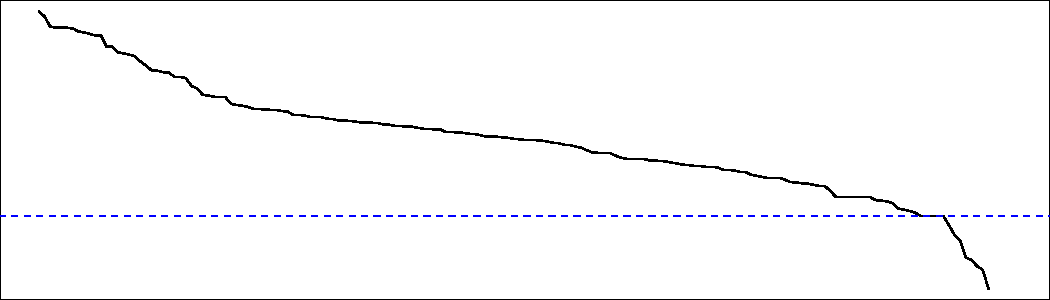
\includegraphics[width=0.8\textwidth]{gmdistraw}%
        \end{figure}


        \column{.28\textwidth}

        \tiny
        \vspace{-30pt}

        \begin{table}[ht]
            \centering
            \begin{tabular}{rr}
                radio/news & 4183 \\ 
                book/info & 1950 \\ 
                TV/news & 1876 \\ 
                radio/music & 1693 \\ 
                speech/informal & 1390 \\ 
                TV/Entertainment & 1000 \\ 
                TV/comedy &  949 \\ 
                speech/discussion &  930 \\ 
                TV/entertainment &  760 \\ 
                email/personal &  575 \\ 
                speech/service &  381 \\ 
                web/social &  286 \\ 
                web/product support &  278 \\ 
                web/comedy/social &  266 \\ 
                music/blues &  248 \\ 
                email/academic &  247 \\ 
                file/documentation &  238 \\ 
                speech/info &  225 \\ 
                web/tech/news &  194 \\ 
                web/tech/reference &  185 \\ 
                web/news &  184 \\ 
                music/folk/metal &  183 \\ 
                web/music &  173 \\ 
                music/progressive &  156 \\ 
                speech/greeting &  150 \\ 
                email/advertising &  149 \\ 
                music/pop &  147 \\ 
                email/orders &  140 \\ 
                web/art &  139 \\ 
                irc/informal/discussion &  132 \\ 
                music/rock &  130 \\
                \ldots & \ldots \\
                % email/business &  129 \\ 
                % web/tech &  124 \\ 
                % web/music/shopping &  120 \\ 
                % music/metal &  119 \\ 
                % music/guitar &  118 \\ 
                % file/ruby code &  117 \\ 
                % web/reference/academic &  103 \\ 
                % web/outdoors/reference &  100 \\ 
                % web/academic/reference &   95 \\ 
                % web/shopping &   91 \\ 
                % web/reference &   90 \\ 
                % speech/ephemera &   90 \\ 
                % music/punk &   86 \\ 
                % web/entertainment &   83 \\ 
                % web/tech/shopping &   81 \\ 
                % web/outdoors &   77 \\ 
                % file/config &   75 \\ 
                % music/fusion &   71 \\ 
                % web/banking &   54 \\ 
                % web/academic &   50 \\ 
                % web/fitness &   45 \\ 
                % web/hosting &   36 \\ 
                % email/technical &   33 \\ 
                % display/output &   32 \\ 
                % web/entertainment/social &   26 \\ 
                % email/spam &   17 \\ 
                % display/interactive &   16 \\ 
                % web/video streaming &   16 \\ 
                % web/search &   15 \\ 
                % sign/product info &   10 \\ 
                % product/packaging &    8 \\ 
                % sign/info/instruction &    8 \\ 
                % sign/info &    6 \\ 
                % sign/advertising &    6 \\ 
                % web/comedy &    3 \\ 
                % web/tech/academic &    0 \\ 
                % music/country/rock &    0  
            \end{tabular}
        \end{table}



        % Raw mean sizes for each genre (all)
% 
%         \begin{table}[ht]
%             \centering
%             \begin{tabular}{rr}
%                 radio/News & 8800 \\ 
%                 speech/Informal & 7200 \\ 
%                 radio/news/entertainment & 5840 \\ 
%                 game/game & 5000 \\ 
%                 TV/documentary & 4800 \\ 
%                 TV/sport & 4800 \\ 
%                 film/Entertainment & 4800 \\ 
%                 game/discussion & 4800 \\ 
%                 phone/informal & 4040 \\ 
%                 radio/News/entertainment & 3600 \\ 
%                 radio/news & 3600 \\ 
%                 speech/discussion/academic & 3600 \\ 
%                 TV/music & 2400 \\ 
%                 video/info/academic & 2400 \\ 
%                 TV/news & 2000 \\ 
%                 book/info & 2000 \\ 
%                 speech/informal/discussion & 1800 \\ 
%                 TV/documentary/entertainment & 1200 \\ 
%                 radio/music & 1200 \\ 
%                 book/ & 1000 \\ 
%                 TV/Entertainment &  800 \\ 
%                 TV/comedy &  800 \\ 
%                 TV/entertainment &  800 \\ 
%                 music/music &  800 \\ 
%                 video/info/advertising &  800 \\ 
%                 speech/Discussion &  520 \\ 
%                 email/personal &  467 \\ 
%                 web/news/tech &  441 \\ 
%                 speech/informal &  400 \\ 
%                 web/games/news &  387 \\ 
%                 web/news/social &  380 \\ 
%                 file/js code &  363 \\ 
%                 music/blues &  306 \\ 
                % speech/info/discussion &  240 \\ 
                % web/reference/shopping &  229 \\ 
                % music/progressive &  200 \\ 
                % flyer/info/advertising &  200 \\ 
                % phone/info &  200 \\ 
                % speech/service/discussion &  200 \\ 
                % web/games &  196 \\ 
                % web/conspiracy &  195 \\ 
                % web/comedy/social &  185 \\ 
                % music/folk/metal &  183 \\ 
                % speech/discussion &  180 \\ 
                % web/news &  179 \\ 
                % web/health &  179 \\ 
                % web/entertainment/images &  172 \\ 
                % web/social &  165 \\ 
                % file/documentation &  161 \\ 
                % speech/Inquiry &  160 \\ 
                % speech/info &  160 \\ 
                % music/pop &  156 \\ 
                % web/music &  153 \\ 
                % web/tech/social &  151 \\ 
                % web/product support &  139 \\ 
                % web/reference/military &  134 \\ 
                % web/music/shopping &  110 \\ 
                % music/metal &  107 \\ 
                % music/pop/metal &  105 \\ 
                % music/punk &  105 \\ 
                % web/academic/reference &  105 \\ 
                % music/guitar &  104 \\ 
                % web/entertainment/news &   99 \\ 
                % music/rock &   99 \\ 
                % web/entertainment &   95 \\ 
                % email/orders &   94 \\ 
                % email/academic &   93 \\ 
                % web/tech/news &   86 \\ 
                % email/advertising &   85 \\ 
                % music/fusion &   81 \\ 
                % speech/ephemera &   80 \\ 
                % speech/greeting &   80 \\ 
                % speech/organisation &   80 \\ 
                % speech/parting &   80 \\ 
                % speech/question &   80 \\ 
                % speech/request &   80 \\ 
                % speech/service &   80 \\ 
                % web/outdoors/reference &   79 \\ 
                % web/reference/academic &   71 \\ 
                % web/tech &   68 \\ 
                % music/country &   66 \\ 
                % web/downloads &   66 \\ 
                % web/entertainment/puzzles &   62 \\ 
                % web/fitness &   61 \\ 
                % web/reference/woodwork &   61 \\ 
                % web/reference &   60 \\ 
                % web/tech/reference &   55 \\ 
                % web/art &   50 \\ 
                % notes/agenda/minutes &   50 \\ 
                % web/info/advert &   50 \\ 
                % web/comedy/entertainment &   49 \\ 
                % file/config &   49 \\ 
                % email/business &   48 \\ 
                % web/reference/travel &   46 \\ 
                % web/tech/utility &   44 \\ 
                % \#N/A &   41 \\ 
                % music/indie &   40 \\ 
                % TV/advertising &   40 \\ 
                % book/packaging/book blurb &   40 \\ 
                % poster/info &   40 \\ 
                % poster/menu &   40 \\ 
                % paper slip/invoice &   37 \\ 
                % file/ruby code &   36 \\ 
                % display/output &   35 \\ 
                % map/info &   35 \\ 
                % web/shopping/investment &   35 \\ 
                % web/outdoors &   32 \\ 
                % file/html code &   31 \\ 
                % application/album listing &   30 \\ 
                % display/info/status &   30 \\ 
                % flyer/advertising &   30 \\ 
                % notes/note &   30 \\ 
                % web/reference/social &   29 \\ 
                % web/entertainment/social &   26 \\ 
                % application/info &   25 \\ 
                % flyer/menu &   25 \\ 
                % sign/instruction &   25 \\ 
                % sign/menu &   25 \\ 
                % sms/info &   25 \\ 
                % irc/informal/discussion &   22 \\ 
                % sms/informal &   21 \\ 
                % TV/advertising/info &   20 \\ 
                % box/address &   20 \\ 
                % card/info &   20 \\ 
                % noticeboard/advert &   20 \\ 
                % web/advertising &   18 \\ 
                % application/info/status &   17 \\ 
                % application/update &   15 \\ 
                % book/packaging/book title &   15 \\ 
                % web/hosting &   14 \\ 
                % email/spam &   13 \\ 
                % email/technical &   13 \\ 
                % poster/advertising &   12 \\ 
                % web/tech/shopping &   10 \\ 
                % application/buttons/info &   10 \\ 
                % display/info &   10 \\ 
                % notes/diagram &   10 \\ 
                % paper slip/info &   10 \\ 
                % sign/map &   10 \\ 
                % sign/product info &   10 \\ 
                % vehicle/branding/sign &   10 \\ 
                % web/utility &    8 \\ 
                % display/interactive &    8 \\ 
                % web/tech/hosting &    8 \\ 
                % sign/info/instruction &    7 \\ 
                % sign/advertising &    7 \\ 
                % TV/info &    6 \\ 
                % sign/advertising/info &    6 \\ 
                % web/banking &    5 \\ 
                % cheque/info &    5 \\ 
                % clothing/packaging &    5 \\ 
                % product/info &    5 \\ 
                % product/instruction/info/packaging &    5 \\ 
                % product/packaging &    5 \\ 
                % sign/ &    5 \\ 
                % sign/info &    5 \\ 
                % taxdisc/info &    5 \\ 
                % web/comedy &    3 \\ 
                % vehicle/info/advertising &    2 \\ 
                % sms/ &    2 \\ 
                % web/reference/entertainment &    1 \\ 
                % web/video streaming &    1 \\ 
                % box/packaging &    1 \\ 
                % web/search &    0 \\ 
                % web/tech/academic &    0 \\ 
                % web/game &    0 \\ 
                % web/blogs &    0 \\ 
                % music/classical &    0 \\ 
                % music/country/rock &    0 \\ 
                % music/electronica &    0 \\ 
                % phone/ &    0 \\ 
                % web/academic &    0 \\ 
                % web/reference/outdoors &    0 \\ 
                % web/shopping &    0  
        %     \end{tabular}
        % \end{table}





    \end{columns}


    \note{}
}






% =============================================================================
\section{Methods/Discussion}
% -----------------------------------------------------------------------------
\subsection*{Findings}
\frame{\frametitle{Observations}
    \begin{itemize}
        \item The spoken/written balance is remarkably even due to broadcast media
            \vspace{5pt}
        \item A million words doesn't `cover much time'
            \vspace{5pt}
        \item Broadcast media dominates spoken word count (50\% vs. BNC's 10\%)
            \vspace{5pt}
        \item Spoken conversations are overrepresented in the BNC (20\% vs. BNC's 40\%)
            \vspace{5pt}
        \item Various categories are `missing' from the BNC
            % {\tiny product labels, music lyrics}
            

        % \item Digital documents require significant post-processing to remove unread content
        %     % markup, or simply bits I don't read of web pages
        %     % most terminal output is unread
        %     % I'm not *always* reading web chat
        % \item Audio needs to be annotated for genre, particpant count, etc. or transcribed
        % \item Pictures require transcription
        % \item Notebook metadata needs tabulating (and, in many cases, completing)
        % \item Web logs need downloading, post-processing
    \end{itemize}
\note{}
}




% Check prelim report
% \frame{\frametitle{Findings --- Linguistic}
% I read a very eclectic mix of things, including:
%             % In one day, for example, I read articles on music theory, a guidebook for climbers, food cooking instructions, brand names on many items of clothing and food, instructions for how to do various things, GPS instructions and maps, and road signs.
%             % This implies that a good representative sample will require a lot more text than first suspected
%             % Low signal-noise ratio: That is, a corpus will have to grow rather large before it includes any whole books, let alone a cross-section of genres.
% 
%             \vspace{10pt}
% \begin{columns}
%     \column{.5\textwidth}
%         \begin{itemize}
%             \item Articles on music theory
%             \item A recipe for boiled sweets
%             \item A Map
%             \item Many brand names
%             % \item ~3 hours of radio 4
%         \end{itemize}
%     \column{.5\textwidth}
%         \begin{itemize}
%             \item p274 of 'Lancashire Rock'
%             \item Inumerable road signs
%             \item Cooking instructions
%             \item Car GPS instructions
%         \end{itemize}
% \end{columns}
% 
% ...and that's only written material.
% 
% \note{}
% }
% 
% \frame{\frametitle{Findings --- Linguistic 2}
% I rarely read \textsl{all} of \textsl{anything}, and often skip:
%             % Correlates with design advice for the web, but I often read only one or two lines of comment
%             \vspace{10pt}
% \begin{itemize}
%     \item Comments on web pages
%             \vspace{10pt}
%     \item Absolutely everything on many web pages
%             \vspace{10pt}
%     \item Almost all content in factual texts
% \end{itemize}
% \note{}
% }
% 
% \frame{\frametitle{Findings --- Linguistic 3}
%     Text can sneak up on you
%     % I find myself subconsciously absorbing text without really actively reading it. This covers things like TV subtitles and quick notes for myself, as well as things like advertising, calendars, branding, etc.
%     % I have to train myself to notice language use
% 
%     \vspace{10pt}
%     \begin{figure}
%         \centering
%         \begin{subfigure}[b]{0.3\textwidth}
%             \centering
%             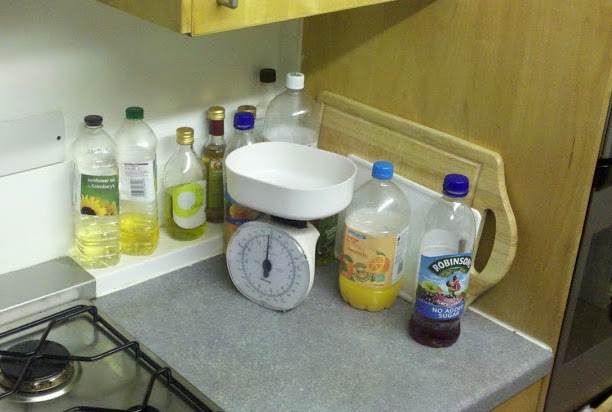
\includegraphics[width=\textwidth]{kitchen}
%         \end{subfigure}%
%         ~ %add desired spacing between images, e. g. ~, \quad, \qquad etc.
%         %(or a blank line to force the subfigure onto a new line)
%         \begin{subfigure}[b]{0.3\textwidth}
%             \centering
%             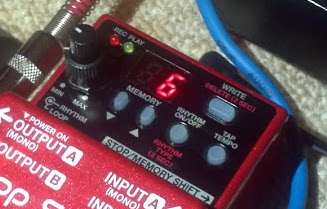
\includegraphics[width=\textwidth]{pedals}
%         \end{subfigure}
%         ~ %add desired spacing between images, e. g. ~, \quad, \qquad etc.
%         %(or a blank line to force the subfigure onto a new line)
%         \begin{subfigure}[b]{0.3\textwidth}
%             \centering
%             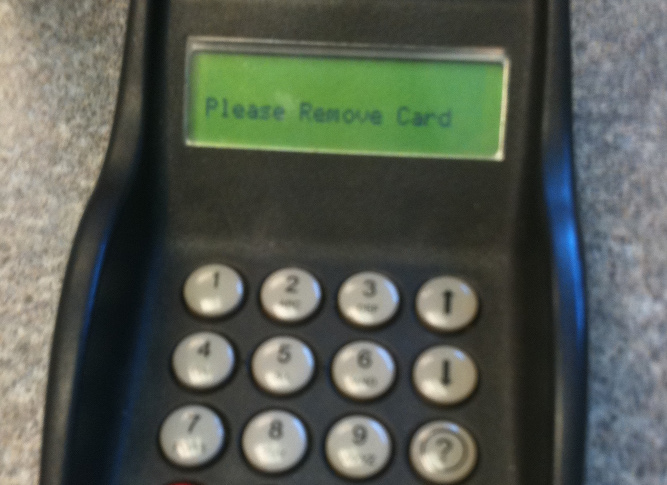
\includegraphics[width=\textwidth]{cpin}
%         \end{subfigure}
%     \end{figure}
% 
%     \vspace{10pt}
%     How many of these do I really \textsl{read} in everyday use?
% 
%     \note{}
% }
% 
% \frame{\frametitle{Findings --- Linguistic 4}
%         I read a very large number of very small texts
%             % contrary to most corpora
%             \vspace{10pt}
% \begin{itemize}
%     \item Typically informative, and 1-2 sentences in length.  
%             \vspace{10pt}
% 
%     \item Many would only read once or twice ever, such as parking machine instructions or button labels
% \end{itemize}
% \note{}
% }
% 
% \frame{\frametitle{Findings --- Linguistic 5}
% Due to radio/music, I often absorb more than one source of text at once
% 
%             \vspace{10pt}
% \begin{itemize}
%     \item Most smaller reading events were done whilst listening to radio 4
%             \vspace{10pt}
%     \item It's unclear how my attention divides itself
% \end{itemize}
%         
% \note{}
% }
% 
% \frame{\frametitle{Findings --- Linguistic 6}
%     The vast majority of text I read is digital, but the vast majority of text sources I read are not.
%             \vspace{10pt}
%     \begin{itemize}
%         \item Caused by my use of news websites, Wikipedia
%             \vspace{10pt}
%         \item Contrasts with my subjective preference for reading `real' books over ebooks
%     \end{itemize}
% 
% \note{}
% }
% 



\frame{\frametitle{Findings --- Methodological}
    \begin{itemize}
        \item Small interactions are hardest to sample
            \vspace{10pt}
        \item Attention models are important (442 word median difference, 5m extra words)
            \vspace{10pt}
        \item Significant manual input still required for many data sources
            \vspace{10pt}
        \item Audio processing is not good enough yet
    \end{itemize}
    \note{}
}





\frame{\frametitle{Findings --- Questions}
    Proper annotation requires a fair amount of procedural knowledge:
    \vspace{10pt}
    \begin{itemize}
        \item How often does one read a document when writing it?
        \item How deliberately must one read something for it to `count'?
        \item What's the best method of recording multiple parallel activities?
        \item What of programming languages, music, numeric and symbolic information, maps, etc.?
    \end{itemize}
    \note{}
}


% -----------------------------------------------------------------------------
\subsection*{Ethics}
\frame{\frametitle{Ethics}
Covert research is always ethically suspect, however:

    \begin{itemize}
        \item Data being captured is not sensitive
        \item There is no other way to capture small spoken utterances
        \item Little to no human listening ever occurs on the resultant data
        \item Automated obfuscation is possible if only taking word counts/proportions
            % such as garbling the speech without affecting frequencies, allowing VAD to still work
        \item Data may be optionally deleted after (nightly) notation in the log 
            % unless sampling verbatim recordings, any data sampled may be deleted after its main points have been
            % noted down.
    \end{itemize}
\note{
  BNC: announced their recordings and allowed for deletion on request
}
}



% -----------------------------------------------------------------------------
% =============================================================================
\section*{Summary}
\frame{\frametitle{Summary}
    \begin{itemize}
        \item Preliminary tests indicate some validity
            \vspace{5pt}
        \item Results from the BNC don't apply to me very well
            \vspace{5pt}
        \item Verbatim text is hard to get, proportions/genres less so
            \vspace{5pt}
        \item Though a single-person sample is useful, multiple people could augment data using questionnaires and data mining

            \vspace{10pt}
        \item My data generalise only to those similar to me!
    \end{itemize}
    \note{}
}



\frame{\frametitle{Further Work}
    \begin{itemize}
        \item Inter-person variance should be identified
            \vspace{10pt}
        \item Further technical additions to tools
            \vspace{10pt}
        \item Automated voice activity detection
            \vspace{10pt}
        \item Better understanding of human attention/interest
            \vspace{10pt}

    \end{itemize}
    \note{}
}



\appendix


% =============================================================================
\section{Variables}

% Which variables are collected
\frame{\frametitle{Variables}
    \begin{itemize}
        \item Source
        \item Title
        \item Medium, Genre (free coded)
        \item Age of document at time of use
        \item Author type (As in Lee's BNC index)
        \item Word count or duration
        \item Spoken/written/interactive
        \item Proportion `used'
        \item Circulation size 
        \item Notes (i.e. times read, any notable properties of context and/or consumption)
    \end{itemize}
\note{}
}






% =============================================================================
% \section{Data Sources}



% -----------------------------------------------------------------------------------------
% 
% \frame{\frametitle{}
% \begin{columns} 
%     \begin{column}[c]{5cm} 
%     \end{column} 
%     \begin{column}[c]{5cm} 
%     \end{column} 
% \end{columns}
% 
% \note{}
% }
%
%
% \frame{\frametitle{}
%     \begin{itemize}
%         \item
%     \end{itemize}
% \note{}
% }
%
% \frame{\frametitle{}
% \note{}
% }
% -----------------------------------------------------------------------------------------
\end{document}
